\section{Sviluppi futuri}
Non tutti i casi d'uso definiti sono stati implementati. Di seguito è riportata una tabella riassuntiva di quali casi d'uso sono stati implementati e quali no.

\begin{table}[h!]
	\centering
	\begin{tabular}{|c|c|c|}
		\hline
		\textbf{Codice} & \textbf{Caso d'uso} & \textbf{Implementato} \\ \hline
		\multicolumn{3}{|c|}{Alta Priorità} \\ \hline
		\textbf{UC1} & Login & Sì\\ \hline
		\textbf{UC2} & Logout & Sì \\ \hline
		\textbf{UC3} & Visualizzazione informazioni account & Sì \\ \hline
		\textbf{UC4} & Visualizzazione informazioni squadra & Sì \\ \hline
		\textbf{UC15} & Inserimento utente & Sì \\ \hline
		\textbf{UC16} & Cancellazione utente & Sì\\ \hline
		\textbf{UC17} & Gestione squadre (creazione) & Sì \\ \hline
		\textbf{UC18} & Visualizzazione informazioni zona & Sì \\ \hline
		\multicolumn{3}{|c|}{Media Priorità} \\ \hline
		\textbf{UC6} & Segnalazione operatività & Sì\\ \hline
		\textbf{UC7} & Visualizzazione intervento di emergenza & No \\ \hline
		\textbf{UC8} & Visualizzazione intervento programmato & No \\ \hline
		\textbf{UC9} & Inserimento informazioni intervento & No \\ \hline
		\textbf{UC11} & Gestione intervento di emergenza & No \\ \hline
		\textbf{UC12} & Gestione intervento programmato & No \\ \hline
		\textbf{UC13} & Gestione report intervento di emergenza & No \\ \hline
		\textbf{UC14} & Gestione report intervento programmato & No \\ \hline
		\textbf{UC20} & Gestione informazioni relative alla zona & No \\ \hline
		\multicolumn{3}{|c|}{Bassa Priorità} \\ \hline
		\textbf{UC5} & Gestione reperibilità & No\\ \hline
		\textbf{UC10} & Visualizzazione posizione real-time & Sì\\ \hline
		\textbf{UC19} & Notifiche allarmi zona & No\\ \hline
	\end{tabular}
	\caption{\label{tab:table-name}Casi d'uso implementati e mancanti.}
\end{table}

\clearpage

\subsection{API Protezione Civile POP}
Di seguito si riporta un esempio di chiamata dell'API Protezione Civile POP che permette di visualizzare alcuni allarmi generati dalla Protezione Civile italiana (\Fig\ref{fig:APIPOP}), presentata nei requisiti ma non implementata in questo progetto. La documentazione è disponibile sul sito \url{https://www.protezionecivilepop.tk/}.

\begin{figure}[h!]
	\centering
	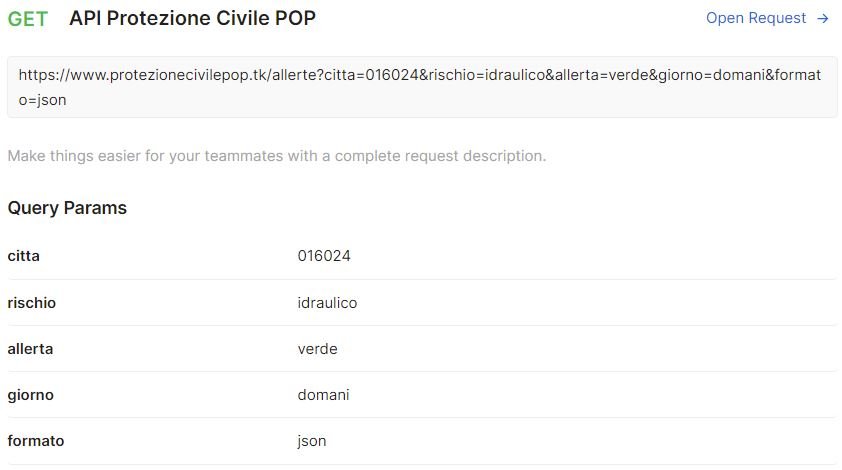
\includegraphics[width=0.95\linewidth]{./Conclusione/ImageFiles/APIProtezioneCivilePOPRequest}
	Response:
	\lstinputlisting[language=json]{./Conclusione/OtherFiles/ProtezioneCivilePOPResponse.json}
	\caption{Documentazione API Protezione Civile POP.}
	\label{fig:APIPOP}
\end{figure}

\clearpage

\subsection{API Terremoti}
Nella figura \ref{fig:APITerremoti} è presentata un esempio di API che permette di visualizzare i terremoti registrati dall'Istituto Nazionale di Geofisica e Vulcanologia, presentata nei requisiti ma non implementata nell'applicazione. La documentazione completa può essere consultata al link \url{https://developers.italia.it/it/api/terremoti-opendata}.

\begin{figure}[h!]
	\centering
	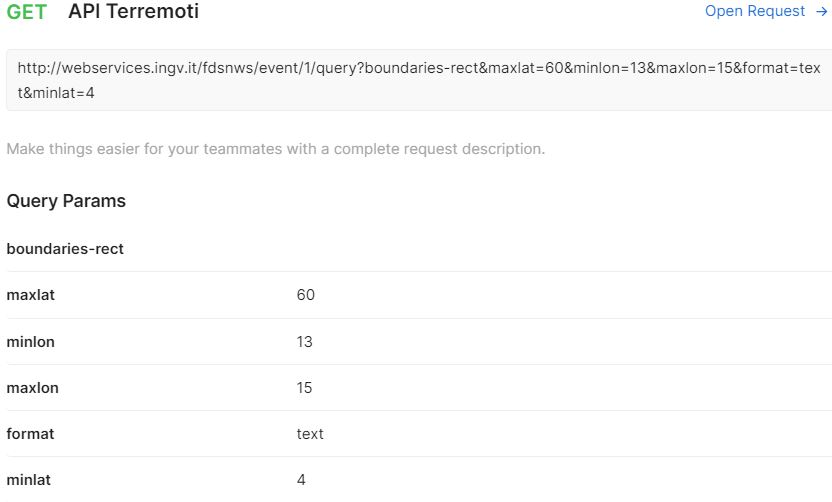
\includegraphics[width=1\linewidth]{./Conclusione/ImageFiles/APITerremotiRequest.JPG}
	
	Response:
	\lstinputlisting[language={}]{./Conclusione/OtherFiles/TerremotoResponse.txt}
	\caption{Documentazione API Terrmoti.}
	\label{fig:APITerremoti}
\end{figure}

\clearpage
